% -*- latex -*-
%%%%%%%%%%%%%%%%%%%%%%%%%%%%%%%%%%%%%%%%%%%%%%%%%%%%%%%%%%%%%%%%
%%%%%%%%%%%%%%%%%%%%%%%%%%%%%%%%%%%%%%%%%%%%%%%%%%%%%%%%%%%%%%%%
%%%%
%%%% This text file is part of the source of 
%%%% `Parallel Programming in MPI and OpenMP'
%%%% by Victor Eijkhout, copyright 2012-8
%%%%
%%%% mpi-gatherscatter.tex : about gather & scatter collectives
%%%%
%%%%%%%%%%%%%%%%%%%%%%%%%%%%%%%%%%%%%%%%%%%%%%%%%%%%%%%%%%%%%%%%
%%%%%%%%%%%%%%%%%%%%%%%%%%%%%%%%%%%%%%%%%%%%%%%%%%%%%%%%%%%%%%%%

\Level 0 {Rooted collectives: gather and scatter}
\label{sec:gatherscatter}

In the \indexmpishow{MPI_Scatter} operation, the root spreads information to
all other processes. The difference with a broadcast is that it involves
individual information from/to every process. Thus, the gather operation typically 
has an array of items, one coming from each sending process, and scatter has an array,
\begin{figure}[ht]
  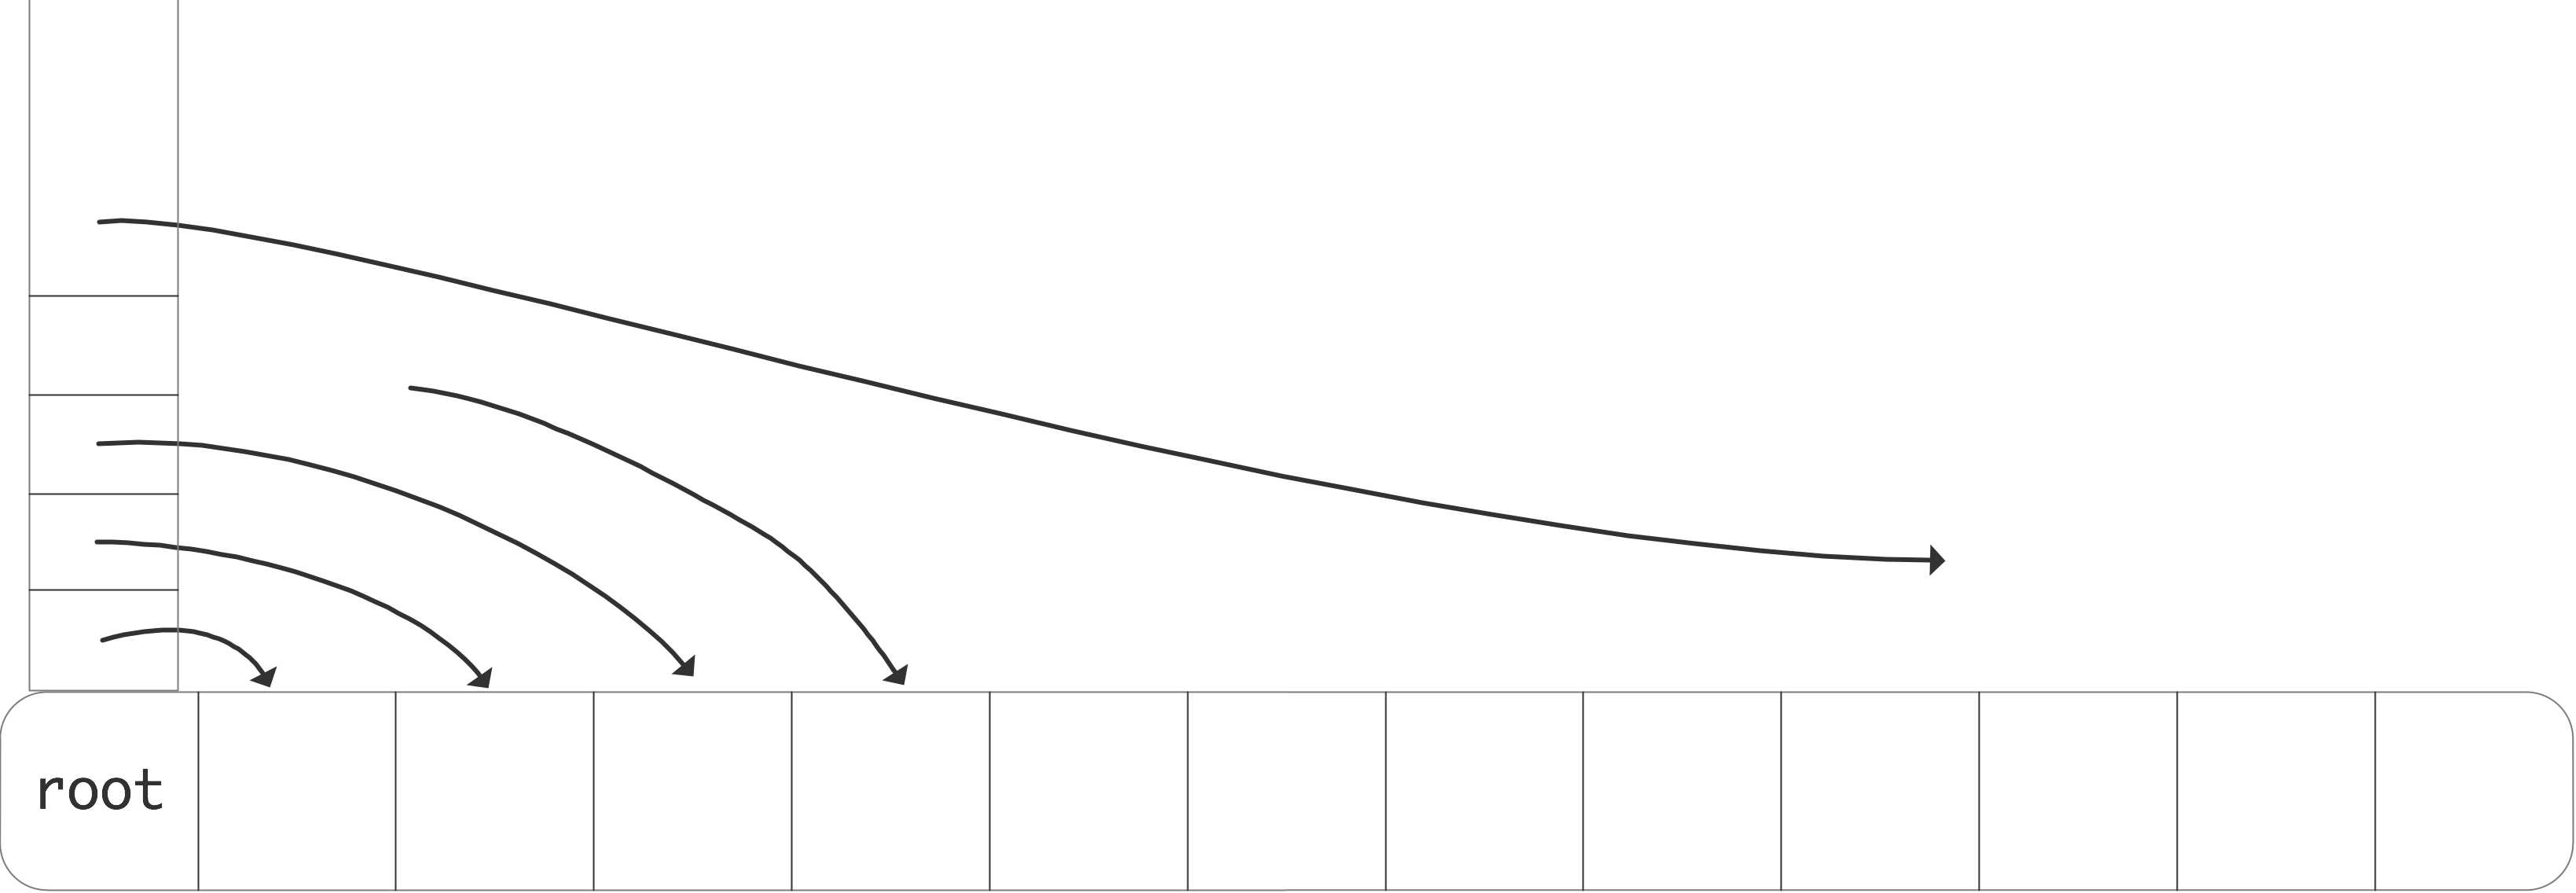
\includegraphics[scale=.12]{graphics/scatter-simple}
  \caption{A scatter operation}
  \label{fig:scatter}
\end{figure}
with an individual item for each receiving process; see figure~\ref{fig:scatter}.

These gather and scatter collectives have a different parameter list from
the broadcast/reduce. The broadcast/reduce involves the same amount
of data on each process, so it was enough to have a buffer, datatype, and size.
In the gather/scatter calls you have
\begin{itemize}
\item a large buffer on the root, with a datatype and size specification, and
\item a smaller buffer on each process, with its own type and size specification.
\end{itemize}
Of course, since we're in SPMD mode, even non-root processes have
the argument for the send buffer, but they ignore it. For instance:
\begin{lstlisting}
int MPI_Scatter
  (void* sendbuf, int sendcount, MPI_Datatype sendtype, 
   void* recvbuf, int recvcount, MPI_Datatype recvtype, 
   int root, MPI_Comm comm) 
\end{lstlisting}
The \n{sendcount} is not, as you might expect, the total length of the
sendbuffer; instead, it is the amount of data sent to each process.

\begin{exercise}
  \label{ex:randomwhere}
  Let each process compute a random number.
  You want to print the maximum value and on what processor it
  is computed. What collective(s) do you use? Write a short program.
\end{exercise}

\Level 1 {Reference}

In the gather and scatter calls, each processor has $n$ elements of individual
data. There is also a root processor that has an array of length~$np$, where $p$
is the number of processors. The gather call collects all this data from the 
processors to the root; the scatter call assumes that the information is 
initially on the root and it is spread to the individual processors.

The prototype for \indexmpishow{MPI_Gather} has two `count' parameters, one
for the length of the individual send buffers, and one for the receive buffer.
However, confusingly, the second parameter (which is only relevant on the root)
does not indicate the total amount of information coming in, but
rather the size of \emph{each} contribution. Thus, the two count parameters
will usually be the same (at least on the root); they can differ if you 
use different \indexmpishow{MPI_Datatype} values for the sending and receiving
processors.

\mpiRoutineRef{MPI_Gather}

Here is a small example:
\cverbatimsnippet[examples/mpi/c/gather.c]{gather}
This will also be the basis of a more elaborate example in
section~\ref{ref:v-collective}.

The \indexmpishow{MPI_IN_PLACE} option can be used for the send buffer on the root;
the data for the root is then assumed to be already in the correct location
in the receive buffer.

The \indexmpishow{MPI_Scatter} operation is in some sense the inverse of the gather:
the root process has an array of length $np$ where $p$~is the number of processors
and $n$~the number of elements each processor will receive.
\begin{lstlisting}
int MPI_Scatter
  (void* sendbuf, int sendcount, MPI_Datatype sendtype, 
   void* recvbuf, int recvcount, MPI_Datatype recvtype, 
   int root, MPI_Comm comm) 
\end{lstlisting}

\Level 1 {Allgather}

The \indexmpishow{MPI_Allgather} routine does the same gather onto
every process.
%
\mpiRoutineRef{MPI_Allgather}

This routine is used in the
%
\indextermsub{dense}{matrix-vector product} to give each processor the
full input; see~\HPSCref{sec:densescaling}.

Some cases look like an all-gather but can be implemented more
efficiently. Suppose you have two distributed vectors, and you want to
create a new vector that contains those elements of the one that do
not appear in the other. You could implement this by gathering the
second vector on each processor, but this may be prohibitive in memory
usage.

\begin{exercise}
  Can you think of another algorithm for taking the set difference of
  two distributed vectors. Hint: look up `bucket-brigade algorithm'
  in~\cite{Eijkhout:IHPSClulu}. What is the time and space complexity
  of this algorithm? Can you think of other advantages beside a
  reduction in workspace?
\end{exercise}
